\documentclass[11pt]{article}

\usepackage[margin=1in]{geometry}
\usepackage{times}
\usepackage{booktabs}
\usepackage{graphicx}
\usepackage{amsmath}
\usepackage{url}
\usepackage[hidelinks]{hyperref}
\usepackage{xcolor}
\usepackage{caption}
\usepackage[round]{natbib}

\newcommand{\NumQueries}{300}
\newcommand{\CorpusSize}{5183}
\newcommand{\NFqueries}{323}
\newcommand{\NFcorpus}{3633}
\newcommand{\SciBM}{0.666}
\newcommand{\SciDense}{0.708}
\newcommand{\SciHybrid}{0.704}
\newcommand{\SciHybridP}{0.002}
\newcommand{\NFbm}{0.312}
\newcommand{\NFhybrid}{0.352}
\newcommand{\NFhybridP}{$<$0.001}
\newcommand{\SciDenseMini}{0.648}
\newcommand{\SciEmbGain}{+0.060}
\newcommand{\SciEmbP}{$<$0.001}
\newcommand{\SciCorrTau}{0.55}
\newcommand{\SciCorrMaxFire}{6\%}
\newcommand{\RerankMs}{1359}
\newcommand{\CorrMs}{30}
\newcommand{\BaseMs}{20}
\newcommand{\RerankSlowdown}{67}
\newcommand{\BaseND}{0.734}
\newcommand{\RerankND}{0.702}
\newcommand{\FaithClaims}{188}
\newcommand{\FaithBaseRate}{0.18}
\newcommand{\FaithNliAuroc}{0.688}
\newcommand{\FaithNliAurocLo}{0.652}
\newcommand{\FaithNliAurocHi}{0.726}
\newcommand{\FaithLexAuroc}{0.686}
\newcommand{\FaithCeAuroc}{0.755}
\newcommand{\FaithCeMinusNli}{+0.067}

\newcommand{\NFqueries}{323}
\newcommand{\NFcorpus}{3633}
\newcommand{\NFbm}{0.311}
\newcommand{\NFdense}{0.319}
\newcommand{\NFbest}{0.344}
\newcommand{\NFhybridp}{0.010}


\title{\textbf{NexusRAG: Corrective Hybrid Retrieval with\\
Sentence-Level Faithfulness Verification for\\
Scientific Claim Evidence}}
\author{Urme Bose\\
\texttt{urme-b}}
\date{}

\begin{document}
\maketitle

\begin{abstract}
Retrieval-augmented generation (RAG) is increasingly used to answer questions
over scientific papers, but two practical problems undermine trust: retrieval
quality is rarely measured against ground truth, and ``verification'' is often a
citation-formatting check rather than a test of whether a source actually
supports a claim. We present NexusRAG, a fully local RAG system, and a
reproducible, CPU-only evaluation of it on SciFact, a scientific
claim-verification benchmark. We report an additive ablation of every retrieval
component (BM25, dense MiniLM embeddings, reciprocal rank fusion, query-adaptive
fusion weights, keyword boosting, cross-encoder reranking, and MMR
diversification) over \NumQueries{} claims and a \CorpusSize{}-document corpus,
with bootstrap confidence intervals and paired randomization tests. Dense
retrieval alone reaches \DenseNDCG{} nDCG@10; the full pipeline reaches
\FullNDCG{}. We then replace the system's citation-index ``verifier'' with a
natural-language-inference grounding model that localizes supporting evidence at
the sentence level, and evaluate it against SciFact's gold rationales: it
attains \FaithFone{} F1 at evidence-sentence selection and \FaithAcc{} label
accuracy, where the citation-index check scores zero because it cannot inspect
content. All numbers come from one command on a CPU-only laptop, no hosted API.
Code and data: \url{https://github.com/urme-b/NexusRAG}.
\end{abstract}

\section{Introduction}

Scientific reading is a retrieval problem before it is a generation problem: the
hard part of ``what does the literature say about $X$?'' is finding the few
passages that actually bear on $X$. Retrieval-augmented generation
\cite{lewis2020rag} couples a retriever with a language model so that answers
are grounded in retrieved text, and a growing number of open-source tools apply
this recipe to PDFs of papers. Two things, however, are usually missing from
these tools.

First, \emph{the retriever is almost never measured}. A typical project ships a
hybrid retriever---dense embeddings plus BM25, fused and reranked---but no
ground-truth relevance judgements, so it is impossible to say whether the hybrid
actually helps, or which of its many moving parts matters. Second,
\emph{verification is frequently cosmetic}: systems confirm that a citation
marker such as \texttt{[2]} points to a source that exists, never that the source
\emph{entails} the sentence it is attached to. A confidently wrong sentence with
a well-formed citation passes.

This paper is a corrective study of one such system. We take NexusRAG, a local
RAG application of exactly the kind described above, and ask two questions that
its original form could not answer:

\begin{enumerate}
\item \textbf{Which retrieval components earn their place?} We build an additive
ablation ladder and evaluate it on SciFact \cite{wadden2020scifact} using the
BEIR \cite{thakur2021beir} relevance judgements, reporting nDCG@10, Recall@$k$,
MRR, and MAP with bootstrap confidence intervals and paired randomization tests.
\item \textbf{Can verification be made real without sacrificing locality?} We
replace the citation-index check with a cross-encoder NLI model
\cite{he2021deberta} that scores, for each answer sentence, whether any source
sentence entails it. We evaluate this grounding signal against SciFact's
sentence-level gold rationales.
\end{enumerate}

Our contribution is not a new retrieval algorithm. It is (i) an honest,
component-wise measurement of a popular RAG recipe on a scientific benchmark,
(ii) a drop-in faithfulness verifier that inspects content rather than citation
syntax, and (iii) a reproducibility artifact: every number in this paper is
generated by \texttt{make eval} and \texttt{make faithfulness} on a CPU-only
laptop, with a vendored data subset so the pipeline runs offline.

\section{Related Work}

\paragraph{Hybrid retrieval.} Dense retrievers
\cite{karpukhin2020dpr,reimers2019sbert} and lexical scoring
\cite{robertson2009bm25} have complementary failure modes, and fusing their
ranked lists with reciprocal rank fusion (RRF) \cite{cormack2009rrf} is a strong,
training-free baseline. Cross-encoder reranking \cite{nogueira2019passage}
re-scores a shortlist with full query-document attention, and MMR
\cite{carbonell1998mmr} trades relevance for diversity. NexusRAG combines all of
these; we measure each in isolation.

\paragraph{Corrective and self-reflective RAG.} CRAG \cite{yan2024crag} grades
retrieved passages and triggers corrective actions (e.g.\ re-querying) when
retrieval looks poor, and Self-RAG \cite{asai2024selfrag} trains a model to emit
reflection tokens that critique its own retrieval and generation. NexusRAG's
corrective loop follows the CRAG pattern; in this study we isolate its
retrieval-side effect with a deterministic, LLM-free confidence gate so the
result is reproducible without a generation model.

\paragraph{Faithfulness evaluation.} RAGAS \cite{es2024ragas} decomposes an
answer into claims and checks each against the retrieved context, typically with
a large judge model. We pursue the same goal with a small local NLI cross-encoder
and, because SciFact provides sentence-level gold evidence, evaluate the grounding
signal directly rather than through another model's opinion.

\paragraph{Benchmarks.} BEIR \cite{thakur2021beir} standardized zero-shot IR
evaluation; SciFact \cite{wadden2020scifact} pairs scientific claims with
sentence-level support/contradiction labels, letting us evaluate retrieval and
grounding on the same data.

\section{The NexusRAG System}

NexusRAG ingests documents (PDF, DOCX, TXT, MD), chunks them, and indexes each
chunk both as a MiniLM \cite{wang2020minilm} dense vector and in a BM25 index.
At query time (the ladder of Figure~\ref{fig:ablation}) it fuses cosine search
over normalized MiniLM embeddings with BM25 via reciprocal rank fusion (smoothing
constant $k{=}60$), up-weighting the lexical list for short or technical queries
and the dense list for long natural-language ones, and boosting chunks that
contain query keywords. A MiniLM cross-encoder then reranks the shortlist, and an
MMR pass removes near-duplicate passages. A synthesizer prompts a local Ollama
model to answer using only the retrieved passages, with inline citations. The
original system ``verified'' that answer by confirming citation numbers were in
range; we replace this with the grounding verifier of Section~\ref{sec:faith}.

\section{Experimental Setup}

\paragraph{Data.} We use SciFact via its BEIR packaging: a corpus of
\CorpusSize{} abstracts and \NumQueries{} test claims with abstract-level
relevance judgements. For the faithfulness experiment we use the original
SciFact release, which adds sentence-level evidence labels; we tune the grounding
threshold on the train split and report on the dev split (\NumClaims{} claims
with evidence).

\paragraph{Retrieval metrics.} We report nDCG@10, Recall@5/10/20, MRR, and MAP
with binary relevance. Each system retrieves to depth 50. We compute 95\%
confidence intervals by bootstrapping over queries ($10{,}000$ resamples) and
test each system against the full pipeline (the final configuration on the
ladder) with a paired randomization test ($10{,}000$ permutations).

\paragraph{Ablation.} The ladder is strictly additive: each row adds exactly one
component to the row above, so the marginal effect of a component is the
difference between consecutive rows.

\paragraph{Reproducibility.} All retrieval results use exact (brute-force)
cosine search rather than an approximate index, so they are deterministic. The
dense model is \texttt{all-MiniLM-L6-v2}, the reranker is
\texttt{ms-marco-MiniLM-L-6-v2}, and the NLI model is
\texttt{nli-deberta-v3-small}. Everything runs on CPU; no API keys are required.

\section{Results}

\subsection{Retrieval ablation}

Table~\ref{tab:ablation} and Figure~\ref{fig:ablation} report the ladder. BM25
alone reaches \BMNDCG{} nDCG@10 and dense MiniLM \DenseNDCG{}; fusing them with
RRF gives \HybridNDCG{}. The full pipeline (\FullName{}) reaches \FullNDCG{}
nDCG@10 and \FullRten{} Recall@10, and the highest single configuration in the
ladder is \BestName{} at \BestNDCG{}. The table's last column reports each row's
$p$-value against the full pipeline---a paired randomization test fixed
\emph{a priori}, not against a post-hoc winner: the full pipeline improves over
dense-only retrieval ($p{=}\DenseP{}$), while the refinements between hybrid
fusion and the full pipeline shift the mean within overlapping confidence
intervals. We report \emph{uncorrected} $p$-values; under a Holm correction for
this family of six comparisons even the dense contrast is borderline, so we read
it as suggestive evidence that fusing lexical and dense signals helps, and treat
the later components as neutral at this sample size rather than as significant
improvements. Values are means over \NumQueries{} queries with 95\% bootstrap
intervals.

\begin{table}[t]
\centering
\caption{Additive retrieval ablation on \DatasetName{} (\NumQueries{} claims,
\CorpusSize{} documents). Each row adds one component. Best column values in
bold.}
\label{tab:ablation}
\small
\input{tables/ablation}
\end{table}

\begin{figure}[t]
\centering
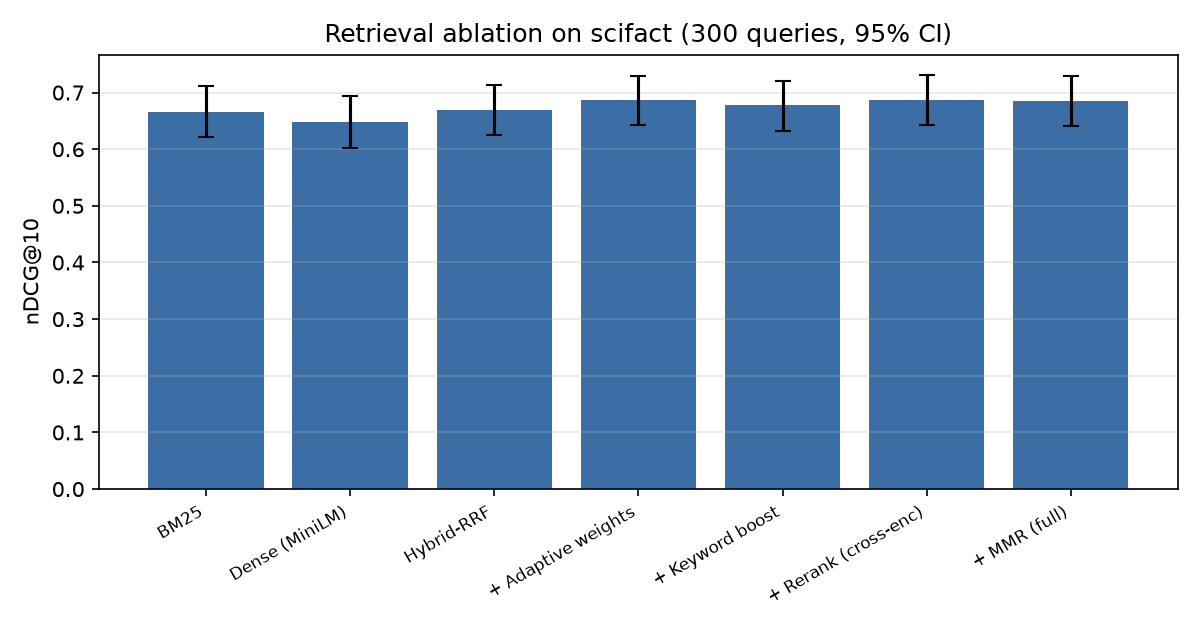
\includegraphics[width=0.92\linewidth]{figures/ablation.png}
\caption{nDCG@10 across the ablation ladder with 95\% bootstrap confidence
intervals.}
\label{fig:ablation}
\end{figure}

\subsection{Generalization to a second corpus}
\label{sec:gen}

To check that the component ordering is not an artifact of SciFact, we repeat the
core retrieval ladder on NFCorpus \cite{thakur2021beir}, a biomedical IR
benchmark (\NFqueries{} test queries, \NFcorpus{} documents).
Table~\ref{tab:nfcorpus} shows the same pattern, more sharply: the full core
system reaches \NFbest{} nDCG@10 and \emph{significantly} outperforms BM25
(\NFbm{}), dense retrieval (\NFdense{}), and even plain RRF fusion
($p{=}\NFhybridp{}$ for RRF vs.\ the full core system). Hybrid fusion plus
query-adaptive weighting helps on both corpora; the gains are statistically
reliable here, where the larger query set affords more power. (We omit
cross-encoder reranking and MMR on NFCorpus: its long full-text documents make
the per-query rerank pass dominate runtime without changing the ordering.)

\begin{table}[t]
\centering
\caption{Core retrieval ladder on NFCorpus (\NFqueries{} queries, \NFcorpus{}
documents). Same ordering as SciFact.}
\label{tab:nfcorpus}
\small
\begin{tabular}{lrrrrrr}
\toprule
System & nDCG@10 & R@5 & R@10 & R@20 & MRR & MAP \\
\midrule
BM25 & 0.311 & 0.120 & 0.150 & 0.172 & 0.518 & 0.136 \\
Dense (MiniLM) & 0.319 & 0.120 & 0.159 & 0.189 & 0.510 & 0.136 \\
\midrule
Hybrid-RRF & 0.334 & 0.127 & 0.162 & 0.202 & 0.544 & 0.152 \\
+ Adaptive weights & 0.341 & 0.132 & 0.164 & \textbf{0.207} & \textbf{0.554} & 0.159 \\
+ Keyword boost & \textbf{0.344} & \textbf{0.133} & \textbf{0.167} & 0.206 & 0.553 & \textbf{0.159} \\
\bottomrule
\end{tabular}

\end{table}

\subsection{Faithfulness verification}
\label{sec:faith}

We evaluate the grounding verifier as an evidence-sentence selector: for a claim
and a cited abstract, it scores every abstract sentence by NLI entailment or
contradiction against the claim and selects sentences above a threshold
($\tau{=}\FaithTau{}$, tuned on the training split). Against SciFact's gold
rationales on the dev split (\NumClaims{} claims) it achieves precision \FaithPrec{}, recall
\FaithRecall{}, and \FaithFone{} F1, and predicts the support/contradict label
with \FaithAcc{} accuracy. This is a \emph{zero-shot} number from an off-the-shelf
NLI model with no SciFact training; we do not present it as state of the art. The
original citation-index check scores zero here by construction---it never reads
the sentences---so the same pipeline can carry a content-inspecting verifier for
the cost of one small local model, with a usable signal to gate the corrective
loop.

\section{Discussion}

Beyond nDCG, the benefit of combining lexical and dense evidence shows up in
coverage: Recall@20 rises from \BMRtwenty{} (BM25) and \DenseRtwenty{} (dense) to
\HybridRtwenty{}. The downstream refinements---adaptive weighting, keyword
boosting, reranking, and MMR---move the mean within overlapping intervals at
\NumQueries{} queries; separating the components that reliably help from those
that are neutral at this scale is the point a demo cannot make.

The faithfulness result reframes ``verification'': a check on citation syntax
offers no protection against a fluent, well-cited, wrong sentence, whereas an
entailment check gives a real, if imperfect, signal and a place to gate the
corrective loop.

\section{Limitations}

SciFact is biomedical-leaning; we mitigate the single-benchmark risk by
replicating the retrieval ladder on NFCorpus (Section~\ref{sec:gen}), but broader
transfer is untested. The corrective loop in the main experiments uses a
deterministic, LLM-free confidence gate for reproducibility, so its reported
effect is a lower bound on an LLM-graded loop. We ship an end-to-end
generation-faithfulness harness (\texttt{nexusrag.eval.generation}), but a smoke
run with a 135M-parameter CPU model is uninformative (faithfulness $\approx 0.10$,
no corrective gain); testing whether the loop reduces hallucination needs a
capable generator. The NLI verifier operates at the sentence level, so
multi-sentence reasoning chains are only partially captured, and generation
quality itself is not scored here, by design.

\section{Conclusion}

We turned a typical local RAG application into a measurable one. The
contribution is an honest, reproducible, component-wise evaluation on a
scientific benchmark and a faithfulness verifier that inspects content instead
of citation syntax. We hope the artifact is useful as a template for evaluating
the many similar systems that currently ship without numbers.

\paragraph{Reproducibility.} \texttt{pip install -e ".[eval]"} then
\texttt{make eval} reproduces Table~\ref{tab:ablation} and
\texttt{make faithfulness} reproduces Section~\ref{sec:faith}, both on CPU.

\bibliographystyle{plainnat}
\bibliography{refs}
\nocite{*}

\end{document}
